\documentclass[10pt,a4paper]{article}



\usepackage[T1]{fontenc}
\usepackage[utf8]{inputenc}
\usepackage{ae}
\usepackage{aecompl}
\usepackage{zefonts}
\usepackage{multicol}
\usepackage{array, multirow, tabularx}
\usepackage{makecell}
\usepackage{graphicx}
% \usepackage{picins}
\usepackage{amsfonts,amsmath,amssymb}
\usepackage{eurosym}
\usepackage{ulem} %permet de barrer sdu texte avec \sout{} , hachurer avec \xout , souligner avec vaguelette \uwave
\usepackage{textcomp}
\usepackage{graphicx}
\usepackage{yhmath} %arc de cercle avec $\wideparen{AB}$
\usepackage[np]{numprint} %espacement grands nombres
\usepackage{fdsymbol} % symbole calculatrice casio
\usepackage{enumerate}
\usepackage{fancybox} % shadowbox etc...
\usepackage{pifont}
\usepackage{tabularx} 
\usepackage{boxedminipage}
\usepackage[thmmarks,framed]{ntheorem}   %fonction  \newtheorem améliorée incompatible avec amsthm
\usepackage{framed}
\usepackage{titlesec}
\usepackage{colortbl} %charge xcolor , à mettre avant tikz sinon conflit...
\usepackage{pgfkeys} % repères avec tikz
\usepackage{tikz}
\usepackage{tkz-tab} %tableaux de variation
\usepackage{esvect} %vecteurs
\usepackage{pgf} %exporter figures geogebra
\usepackage{mathrsfs} %exporter figures geogebra
\usepackage{slashbox} %sépare une cellule en 2 dans un tableau \backslashbox{Texte dessous}{Texte dessus}
\usepackage{diagbox} %\diagbox{}{}
\usetikzlibrary{arrows} %exporter figures geogebra
\usepackage[french,frenchkw,algoruled]{algorithm2e} %algo 
%\usepackage{algorithm} %algo style algobox
% \usepackage{algpseudocode}% algo style algobox
% \input algtolatex %algo style algobox - nécessite le fichier algolatex.
\usepackage{calrsfs} % plus belles majuscules avec \mathcal
% \usepackage{sesamanuel} % pour les commandes spéciales du manuel 2de
% \usepackage{sesamanuelTIKZ} % pour les commandes spéciales de la figure
%\usepackage{stmaryrd} %double crochet avec \llbracket et rrbracket$
\usepackage{qrcode} %qrcode cliquable \qrcode[height=taille]{adresse}
\usepackage{hyperref} %lien hypertexte \href{adresse}{texte}
%\usepackage[xcas]{pro-graphes} %graphe and co
%\usepackage{dijkstra}
\usepackage{tcolorbox} %cadres plus jolis
\usepackage{karnaugh-map} %permet de tracer des tableaux de Karnaugh
%\usepackage{graphicx}
\usepackage[export]{adjustbox} % Alignement vertical images avec b,t,c \includegraphics[scale=1,valign=t]{Image.png}
\usepackage{fancyvrb} % verbatim amélioré \begin{Verbatim}[frame=single,label=,numbers=left] etc [frame=single/leftline/topline/bottomline/lines] framerule=1mm framesep=5mm rulecolor=\color{red} fillcolor=\color{yellow}
\usepackage[load-configurations = abbreviations]{siunitx}
%\sisetup{locale = FR,detect-all,inter-unit-product= \cdot} %norme SI pour les nombres et unités 
%\SI{25000}{mm} \SI{6.022e23}{\per\mol}  \SI{300}{\watt\per\square\meter} \SI{300}{W / m^2} \SI[per-mode=symbol]{210}{\km\per\hour}
% unité seule \si{\newton\meter} nombre seul \num{24415.15625}

\usepackage{witharrows} %permet de mattre des flèches entre lignes d'équations \begin{WithArrows}@ \Arrow{@}\\@\end{WithArrows}

\usepackage{xlop} % pose les oprétaions "à la main" \opadd{@}{@}; opsub ; opmul ; opdiv (eucl) ; opidiv
%\usepackage{minted}{Python} % permet d'écrire en Python avec \begin{minted}{Python}@\end{minted}
\usepackage{stmaryrd} % crochets intervalles entiers \llbracket ; \rrbracket ; parall \sslash ; contradiction \lightning

\usepackage{mathtools}

%%%%%%%Compteurs%%%%%%%%%%%%%%%%%%%%%%%%%%%%%%%%%%%%%%%%%%%%%%%%%%%%%%%%%%%%%%%%%%%%%
% \newcounter{defcompt}   %Défintion d'un compteur
% \newcounter{exocompt}
% \newcounter{theocompt}
% \newcounter{propcompt}
% \newcounter{regcompt}
\newcounter{numexos}

\setcounter{numexos}{0} %initialisation du compteur





% Nouvelles commandes
\definecolor{cqcqcq}{rgb}{0.7529411764705882,0.7529411764705882,0.7529411764705882} %gris geogebra

\newcommand{\paral}{~\mathbin{\!/\mkern-5mu/\!}~} % symbole parallèle

\newcommand{\R}{\mathbb{R}}
\newcommand{\N}{\mathbb{N}}
\newcommand{\D}{\mathbb{D}}
\newcommand{\Z}{\mathbb{Z}}
\newcommand{\Q}{\mathbb{Q}}
\newcommand{\C}{\mathbb{C}}
\newcommand{\U}{\mathbb{U}}

\newcommand{\rel}{\mathcal{R}} % relation binaire

\newcommand{\e}{\text{e}} % exponentielle en lettre droite dans $$ 

\newcolumntype{R}[1]{>{\raggedleft\arraybackslash }b{#1}}
\newcolumntype{L}[1]{>{\raggedright\arraybackslash }b{#1}}
\newcolumntype{C}[1]{>{\centering\arraybackslash }b{#1}}

\newcolumntype{G}[1]{>{\raggedright\arraybackslash }X{#1}}
\newcolumntype{D}[1]{>{\raggedleft\arraybackslash }X{#1}}
\newcolumntype{M}[1]{>{\centering\arraybackslash }X{#1}}


\newcommand{\exe}{\textbf{Exemple : }}
\newcommand{\exes}{\textbf{Exemples : }}
\newcommand{\rema}{\textbf{Remarque : }}
\newcommand{\rems}{\textbf{Remarques : }}
\newcommand{\rap}{\textbf{Rappel : }}
\newcommand{\raps}{\textbf{Rappels : }}
\newcommand{\dem}{\textbf{Démonstration : }}
\newcommand{\dems}{\textbf{Démonstrations : }}
\newcommand{\csq}{\textbf{Conséquence : }}







\newcommand{\Ex}[1]{{\sc{Exercice #1:}}}
\newcommand{\defi}[1]{\begin{leftbar}
\textbf{Définition :} {#1}
 \end{leftbar}}
\newcommand{\defis}[1]{\begin{leftbar}
\textbf{Définitions :} {#1}
 \end{leftbar}}
 
\newcommand{\prop}[1]{\begin{framed}
\textbf{Propriété :} {#1}
 \end{framed}} 
 
\newcommand{\props}[1]{\begin{framed}
\textbf{Propriétés :} {#1}
 \end{framed}} 
 
\newcommand{\theo}[1]{\begin{framed}
\textbf{Théorème :} {#1}
 \end{framed}} 
\newcommand{\theos}[1]{\begin{framed}
\textbf{Théorèmes :} {#1}
 \end{framed}}  
 
\newcommand{\reg}[1]{\begin{framed}
\textbf{Règle :} {#1}
 \end{framed}} 
\newcommand{\regs}[1]{\begin{framed}
\textbf{Règles :} {#1}
 \end{framed}}  
 
\newcommand{\propdef}[1]{\begin{framed}
\textbf{Propriété - Définition :} {#1}
 \end{framed}} 
\newcommand{\propsdef}[1]{\begin{framed}
\textbf{Propriétés - Définition :} {#1}
 \end{framed}}  
 
 
 \newcommand{\csqs}[1]{\begin{framed}
 \textbf{Conséquences :} {#1}
 \end{framed}} 
 
\newcommand{\cor}[1]{\begin{framed}
\textbf{Corollaire :} {#1}
 \end{framed}}     
     
     
%\newcommand{\cadre}[2]{
%\begin{tcolorbox}[colback=red!5!white,
%                  colframe=red!75!black,
%                  title={#1}]
%{#2}
%\end{tcolorbox}  }

\newcommand{\cadre}[3]{
\begin{tcolorbox}[colback=#1!5!white,
                  colframe=#1!75!black,
                  title={#2}]
{#3}
\end{tcolorbox}  }




\newcommand*{\Coord}[3]{% 
\ensuremath{\vv{#1}\, 
    \begin{pmatrix} 
      #2\\ 
      #3 
    \end{pmatrix}}} % coordonnées de vecteurs.
    
\newcommand{\fonction}[5]{\begin{tabular}[t]{cccc}
$#1 :$ & $#2$ & $\longrightarrow$ & $#3$ \\
 & $#4$ & $\longmapsto$ & $#5$
\end{tabular}}
    
\newcommand{\att}{{\fontencoding{U}\fontfamily{futs}\selectfont\char 66\relax \quad}}    % symbole attention

\newcommand{\exo}{%Création d'une macro ayant un paramètre
\addtocounter{numexos}{1}%chaque fois que cette macro est appelée, elle ajoute 1 au compteur numexos
{\sc{Exercice\,\thenumexos\,:}}\,%la valeur du compteur appelée par \thenumeexos
}

\newcommand{\bint}{\displaystyle \int\limits} %signe intégral plus grand

\newcommand{\bsum}{\displaystyle \sum} %signe somme plus grand

\newcommand{\bprod}{\displaystyle \prod\limits} %signe produit plus grand

\newcommand*{\norme}[1]{\left\lVert\vv{#1}\right\rVert}  %norme de vecteur

\newcommand{\ps}[2]{\ensuremath{\vv{#1}.\vv{#2}}} %produit scalaire

\newcommand{\x}{\times} %produit

\newcommand{\modulo}{\text{ modulo }} 

\renewcommand{\Im}[1]{\text{Im} (#1)}

\renewcommand{\Re}[1]{\text{Re} (#1)}

\newcommand{\modu}[3]{{#1} \equiv {#2} ~ [{#3}]}


\newcommand*{\sep}[1]{
\dotfill
\vspace*{-0.3cm}
\begin{center}
\textbf{#1}
\end{center}
\vspace*{-0.5cm}
\dotfill}


%Flèches avec commentaire : exemple $\xRightarrow[test1]{test1}$
%\makeatletter
%\newcommand{\xRightarrow}[2][]{\ext@arrow 0359\Rightarrowfill@{#1}{#2}}
%\makeatother
%
%\makeatletter
%\newcommand{\xLeftarrow}[2][]{\ext@arrow 0359\Leftarrowfill@{#1}{#2}}
%\makeatother
%
%\makeatletter
%\newcommand{\xLeftrightarrow}[2][]{\ext@arrow 0359\Leftrightarrowfill@{#1}{#2}}
%\makeatother


% Renouvellement commandes

\renewcommand{\leq}{\leqslant}
\renewcommand{\geq}{\geqslant}
\renewcommand{\thesection}{\Roman{section} )  \hspace{-4mm}}
\renewcommand{\thesubsection}{\quad \arabic{subsection}\hspace{-0.9mm} ) \hspace{-5mm}}
\renewcommand{\thesubsubsection}{\qquad \alph{subsubsection}\hspace{0.5mm} ) \hspace{-5mm}}


% Présentation générale

\newcommand{\titre}[1]{\begin{center} \Large \sc \fbox{{#1}}\end{center}}

\newcommand{\entete}[1]{\begin{center} \large \underline{#1} \end{center}}

\titleformat*{\section}{\large\bfseries}
\titleformat*{\subsection}{\large\bfseries}
\titleformat*{\subsubsection}{\large\bfseries}
\titleformat*{\paragraph}{\large\bfseries}
\titleformat*{\subparagraph}{\large\bfseries}

%\newcommand{\DS}[3]{\begin{tabular}{|L{6cm}|C{5cm}|C{6cm}|}
%\hline 
%Nom : & Devoir Surveillé #1 & Classe \quad :\quad #2 \\ 
%Prénom : &  & #3 \\ 
%\hline 
%\end{tabular} }

\newcommand{\DS}[3]{\begin{tabularx}{1 \linewidth}{|G|M|M|}
\hline 
Nom : & Devoir Surveillé #1 & Classe \quad :\quad #2 \\ 
Prénom : &  & #3 \\ 
\hline 
\end{tabularx} }

\newcommand{\DSBTS}[4]{\begin{tabularx}{1 \linewidth}{|G|M|M|}
\hline 
Nom : & Devoir Surveillé #2 & Classe \quad :\quad #3 \\ 
Prénom : & #1 & #4 \\ 
\hline 
\end{tabularx} }

\newcommand{\DM}[3]{\begin{tabular}{|L{6.1cm}|C{5.6cm}|C{6.1cm}|}
\hline 
Nom : & Devoir à la maison~ #1 & Classe \quad :\quad #2 \\ 
Prénom : &  & Pour le #3 \\ 
\hline 
\end{tabular} }

\newcommand{\ct}[3]{\begin{tabular}{|L{6.1cm}|C{5.6cm}|C{6.1cm}|}
\hline 
Nom : & Contrôle~ #1 & Classe \quad :\quad #2 \\ 
Prénom : &  & #3 \\ 
\hline 
\end{tabular} }

% Repères automatisés avec Tikz 
% Définition des nouvelles options xmin, xmax, ymin, ymax
% Valeurs par défaut : -3, 3, -3, 3
\tikzset{
xmin/.store in=\xmin, xmin/.default=-3, xmin=-3,
xmax/.store in=\xmax, xmax/.default=3, xmax=3,
ymin/.store in=\ymin, ymin/.default=-3, ymin=-3,
ymax/.store in=\ymax, ymax/.default=3, ymax=3,
}
% Commande qui trace la grille entre (xmin,ymin) et (xmax,ymax)
\newcommand {\grille}
{\draw[help lines] (\xmin,\ymin) grid (\xmax,\ymax);}
% Commande \axes
\newcommand {\axes} {
\draw[->] (\xmin,0) -- (\xmax,0);
\draw[->] (0,\ymin) -- (0,\ymax);
}
% Commande qui limite l’affichage à (xmin,ymin) et (xmax,ymax)
\newcommand {\fenetre}
{\clip (\xmin,\ymin) rectangle (\xmax,\ymax);}

% Exemple 
%\begin{center}
%\begin{tikzpicture} [xmin=@,xmax=@,ymin=@,ymax=@]
%\grille \axes \fenetre
%\draw plot[smooth] (\x,@);
%\end{tikzpicture}
%\end{center}

%%%%%%%\newtheorem{}{×}%%%%%%%%%%%%%%%%%%%%%%%%%%%%%%%%%%%%%%%%%%%%%%%%%%%%%%%%%%%%%
%\theoremseparator{\hspace{0.8mm} :}
%{\theoremseparator{~:}
%\newtheorem*{rem}{Remarque}
%\newtheorem*{rems}{Remarques}
%\newframedtheorem{theo}[theocompt]{Théorème}
%\newtheorem{prop}[propcompt]{Propriété}
%\newtheorem{regle}[regcompt]{Règle}
%\newtheorem{defi}[defcompt]{Définition}
%\newtheorem*{voc}{Vocabulaire}}


%algo
%VARIABLES : 
%\Variables
%Début et fin de bloc :
%\DebutAlgo 
%\FinAlgo 
%\DebutPour
%\FinPour
%\DebutTantQue
%\FinTantQue
%\DebutSi
%\FinSi
%\DebutSinon
%\FinSinon
%SI...ALORS :
%\Si{(...)}
%SINON :
%\Sinon
%POUR ... ALLANT_DE ... A ...
%\Pour{...}{...}{...}
%TANT_QUE(...)
%\Tantque{(...)}
%Pour toutes les autres instructions (y compris les déclarations de variable)
%\Ligne ...


% Mise en page
\usepackage[left=1cm, right=1cm, top=1cm , bottom=1cm]{geometry}
\pagestyle{empty} % pas de numéro de page
\renewcommand{\arraystretch}{1.5} %hauteur des lignes dans un tableau
\setlength{\parindent}{0pt} % pas de retrait de paragraphe

%\usepackage[left=1cm, right=1cm, top=-0.5cm , bottom=1cm,includeheadfoot]{geometry}
%\usepackage{fancyhdr}
%\pagestyle{fancy}

%\renewcommand{\headrulewidth}{1pt}
%\fancyhead[C]{\textbf{page \thepage}} 
%\fancyhead[L]{\leftmark}
%\fancyhead[R]{machin}

%\renewcommand{\footrulewidth}{1pt}
%\fancyfoot[C]{\textbf{page \thepage}} 
%\fancyfoot[L]{truc}
%\fancyfoot[R]{\leftmark}

% \tikz[baseline=(letter.base)]\node[draw,circle,inner sep=1pt] (letter) {B} %lettre entourée



\begin{document}


\titre{Matrices et opérations élémentaires}


\section{Généralités}

\defi{Une \textbf{matrice} de taille $n \x p$ est un tableau de $n$ lignes et $p$ colonnes composé de nombres réels appelés les coefficients de la matrice.

Une telle matrice s'écrit sous la forme  $A=$ \bordermatrix{
   & C_1 & C_2 & \dots & C_{p-1} & C_p \cr 
 L_1 & a_{1,1} & a_{1,2} & \dots & a_{1,p-1} & a_{1,p} \cr
 L_2 &  a_{2,1} & a_{2,2} & \dots & a_{2,p-1} & a_{2,p} \cr
 \vdots &  \vdots &  \vdots &  \ddots &  \vdots &  \vdots \cr 
 L_{n-1} &  a_{n-1,1} & a_{n-1,2} & \dots & a_{n-1,p-1} & a_{n-1,p} \cr
 L_n &  a_{n,1} & a_{n,2} & \dots & a_{n,p-1} & a_{n,p} \cr 
 }
 
On note $A=(a_{(i;j)})$ ou $A=(a_{ij})$ lorsqu'il n'y pas de confusion possible.

Le \textbf{coefficient $a_{ij}$} est celui situé à la ligne $i$ ($L_i$) et la colonne $j$ ($C_j$) de la matrice. (avec $i \in \llbracket 1;n \rrbracket$ et $j \in \llbracket 1;p \rrbracket$).

L’ensemble des matrices de dimensions $n \x p$ est noté $\mathcal{M}_{n,p}(\R)$.
}


\exe $A=\begin{pmatrix}
1&2&3 \\
-1&4&5 
\end{pmatrix}$ est une matrice de taille $2 \x 3$ où $a_{13}=3$ et $a_{21}=-1$.

\defis{ 
\begin{enumerate}[$\bullet$]
\item Une matrice de taille $n \x n$ est appelée une \textbf{matrice carrée} d'ordre $n$.

L'ensemble des matrices carrées d'ordre est noté $\mathcal{M}_{n}(\R)$.

Pour une matrice carrée $A=(a_{ij})$ d'ordre $n$ , l'ensemble des coefficients de la \textbf{diagonale principale} est :
$\{ a_{ii} ; 1 \leq i \leq n\}$.
\item On appelle \textbf{matrice diagonal}e d'ordre $n$ toute matrice carrée d'ordre $n$ telle que tous ses coefficients hors de la diagonale principale valent 0.

\item Une matrice de dimension $1 \x p$ est appelée \textbf{matrice ligne}.

Une matrice de dimension $n \x 1$ est appelée \textbf{matrice colonne}.

\end{enumerate}

}

\exes $B=\begin{pmatrix}
1&2 \\
-1&4 
\end{pmatrix}$ est une matrice carré d'ordre 2.

$C=\begin{pmatrix}
1&0&0 \\
0&-34&0 \\
0&0&7 \\ 
\end{pmatrix}$ est une matrice diagonale d’ordre 3.


$D=\begin{pmatrix}
1&8&-5 \end{pmatrix}$ est une matrice ligne de dimension $1 \x 3$.

Les coordonnées d'un vecteur du plan est une matrice colonne de dimension $2 \x 1$.

\prop{Deux matrices $A =(a_{ij})$ et $B=(b_{ij})$ de même dimension $n \x p$ sont égales si, et seulement si :

$a_{ij} = b_{ij}$ pour tous $i \in \{1 ; 2 ; ... ; n\}$ et $j \in \{1 ; 2 ; ... ; p\}$.

}




\section{Opérations}

\subsection{Somme de deux matrices}

\defi{Soit $A$ et $B$ deux matrices de même taille.

La somme de $A$ et $B$ est la matrice, notée $A+B$ , dont les coefficients sont obtenus en additionnant deux à deux des coefficients qui ont la même position dans $A$ et $B$.}

\exe $A=\begin{pmatrix} 1&5 \\ -1&3  \end{pmatrix}$ et $B=\begin{pmatrix} 4&-1 \\ 8&2  \end{pmatrix}$. 
On a $C=A+B=\begin{pmatrix} 1+4&5+(-1) \\ -1+8&3+2  \end{pmatrix}=\begin{pmatrix} 5&4 \\ 7&5  \end{pmatrix}$.

\rema Il n'est possible d'additionner que des matrices de même dimension.

\props {Soient $A, B$ et $C$ trois matrices de même dimension $n \x p$.
\begin{enumerate}[\quad $\bullet$]
\item (Commutativité de l'addition) : $A + B = B + A$.
\item (Associativité de l'addition) : $(A + B) + C = A + (B + C) = A + B + C.$
\item (Élément neutre de l'addition) : On note $0_{n,p}$ la matrice nulle de dimension $n \x p$ dont tous les coefficients sont nuls. On a $A + 0_{n,p} = A$.
\end{enumerate}
}

\subsection{Produit d'une matrice par un réel}

\defi{Soit une matrice $A$ et un nombre réel $k$.

La produit de $A$ par le réel $k$ est la matrice, notée $kA$, dont les coefficients sont obtenus en multipliant tous les coefficients de $A$ par $k$.}

\exe Soit $A=\begin{pmatrix} 1&5 \\ -1&3  \end{pmatrix}$. On a $7A=\begin{pmatrix} 7\x1&7\x5 \\ 7\x(-1)&7\x3  \end{pmatrix}
=\begin{pmatrix} 7&35 \\ -7&21  \end{pmatrix}$.

\props {Soit $A$ et $B$ deux matrices carrées de même taille et deux réels $k$ et $k'$.
\begin{multicols}{2}
\begin{enumerate}[$\bullet$]
\item  $(k+k')A=kA+k'A$
\item $k(A+B)=kA+kB$
\item $(kk')A=k(k'A)$
\item $kA = 0_{n,p}$ si, et seulement si, $k = 0$ ou $A = 0_{n,p}$.
\end{enumerate}
\end{multicols}
}


\dem Dernière propriété (sens direct): $kA = 0_{n,p} \iff \forall i \in \llbracket 1;n \rrbracket, \forall j \in \llbracket 1;p \rrbracket ,ka_{ij}=0$. 

Or $ka_{ij}=0 \iff k=0$ ou $a_{ij}=0$.

Par disjonction de cas :

$\bullet$ Si $k \neq 0$ alors $\forall i \in \llbracket 1;n \rrbracket, \forall j \in \llbracket 1;p \rrbracket a_{ij}=0$ i.e. $A=0_{n,p}$.

$\bullet$ Si $k=0$ l'implication est trivialement vérifiée.


\subsection{Produit de deux matrices}

\defi{Soit $A = (a_{ij} )$ une matrice de dimension $n \x p$ et $B = (b_{ij} )$ une matrice de dimension $m \x q$.

Le produit matriciel $AB$ est défini si, et seulement si, $p = m$.

Alors $AB = (p_{ij})$ où $p_{ij}= \bsum_{k=1}^p a_{ik}b_{kj}$ pour tous $i \in \{1 ; 2 ; ... ; n\}$ et $j \in \{1 ; 2 ; ... ; q\}.$.

}

\begin{center}
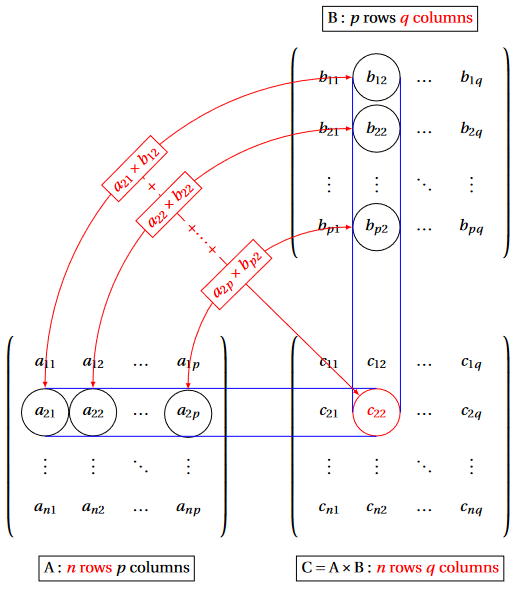
\includegraphics[width = 0.4 \linewidth]{prod_mat}
\end{center}

\exe Soient $A=\begin{pmatrix}   5&2\\-1&3   \end{pmatrix}$ et $B=\begin{pmatrix}   4&-7\\6&1  \end{pmatrix}$. Calculons $AB$. 

$\begin{array}{cc}
 & \begin{pmatrix}
   4  &-7  \\6  &1
  \end{pmatrix}
\\
  \begin{pmatrix}
   5&2\\-1&3
  \end{pmatrix}
 &
  \begin{pmatrix}
   c_{11}& c_{12} \\ c_{21}& c_{22}
  \end{pmatrix}
\end{array}$
avec $\left\lbrace \begin{array}{l} c_{11}=5\x 4 +2 \x 6 = 32 \\
c_{12}=5\x (-7) +2 \x 1 = -33  \\ 
c_{21}=-1\x 4 + 3 \x 6 = 14	\\
 c_{22}=-1\x (-7) + 3 \x 1 = 10	\\
 \end{array} \right.$
 
Finalement $AB=\begin{pmatrix}   32&-33\\14&10   \end{pmatrix}$.

On trouve $BA=\begin{pmatrix}   27&-13\\29&15  \end{pmatrix}$.

\rema \raisebox{-3.5mm}{\shadowbox{La multiplication de matrices n'est pas commutative}}. Sur l'exemple précédent on voit bien que $AB \neq BA$.


\props {Soient $A, B$ et $C$ trois matrices et soit $k$ un nombre réel.

Les propriétés suivantes sont valables sous réserve que les calculs soient possibles.

\begin{enumerate}[$\quad \bullet$]
\item (Associativité de la multiplication) : $(AB)C=A(BC)=ABC$.
\item (Distributivité de la multiplication) : $A(B+C)=AB+AC$ et $(A+B)C=AC+BC$
\item $(kA)B=A(kB)=k(AB)=kAB$
\item (Élément absorbant) : $0_{m,n}A=0_{m,p} $ et $A0_{p,m}=0_{n,m}$
\end{enumerate}
}



\section{Matrice inverse}

\subsection{Matrice unité ou matrice identité}

\defi{On appelle matrice unité ou matrice identité de taille $n \in \N^*$ la matrice carrée formée de $n$ lignes et $n$ colonnes, tel que :

$I_n=\begin{pmatrix}
1&0&\dots&0\\  
0&1&\dots&0\\    
\vdots  & \vdots &\ddots&0\\  
0&0&\dots&1\\   
\end{pmatrix}$

}

\rema La matrice unité est une matrice carrée avec des 1 sur la diagonale et 0 des partout ailleurs.


\prop{ (Élément neutre de la multiplication) : Pour toute matrice carrée $A$ de taille $n$ , on a :
$A \x I_n = I_n \x A =A$ }

\exe Calculer $A \x I_2$ et $I_2 \x A$ avec $A = \begin{pmatrix}   7&-1\\2&5  \end{pmatrix}$.

\subsection{Puissance d'une matrice carrée}

\defi{Soit $A$ une matrice carrée et $n$ un entier naturel non nul.

La puissance n$^{ième}$ de $A$ est la matrice, notée $A^n$, égale au produit de $n$ facteurs $A$.}

\rems
\begin{enumerate}[$\bullet$]
\item$A^0=I_n ; A^1=A$
\item Le carré de $A$ est la matrice, noté $A^2$, égale à $A \x A$.
\item Le cube de $A$ est la matrice, noté $A^3$, égale à $A \x A \x A$.

\end{enumerate}




\exes
\begin{enumerate}[a)]
\item  Soit $A=\begin{pmatrix}   3&-1\\2&1  \end{pmatrix}$. Calculer $A^2$ puis $A^3$.
\item Soit la matrice diagonale $C=\begin{pmatrix} 1&0&0 \\ 0&2&0 \\ 0&0&3 \\ \end{pmatrix}$. Calculer $A^2$.

\rema On constate que tous les coefficients qui ne se trouvent pas sur la diagonale s'annulent et que sur la diagonale, les coefficients de $A^2$ sont égaux aux carrées des coefficients de $A$.

On peut généraliser cette règle à une puissance quelconque.

Ainsi on a par exemple $A^5=$
\end{enumerate}

\subsection{Matrice inverse d'une matrice carrée}

\defi{Une matrice carrée $A$ de taille $n$ est une \textbf{matrice inversible} s'il existe une matrice $B$ telle que :


$A \x B = B \x A = I_n$.

La matrice $B$ notée $A^{-1}$ est appelée la matrice inverse de $A$.
}

\rema Si elle existe la matrice inverse est unique.

\dem Supposons qu'il existe $B$ et $B'$ avec $B \neq B'$ telles que $\left\lbrace \begin{array}{l} AB=BA=I \\ AB'=B'A=I \end{array} \right.$

Alors $AB=I \xRightarrow{\x \text{à gauche}} B'(AB)=B'I \iff (B'A)B=B' \iff B=B'$. Ce qui contredit notre hypothèse de départ.


\exe Soient $A=\begin{pmatrix}   1&-2\\-3&7  \end{pmatrix}$ et $B=\begin{pmatrix}   7&2\\3&1  \end{pmatrix}$.

On a $AB=BA=I_2$

Les matrices $A$ et $B$ sont donc inverses l'une de l'autre et $B=A^{-1}$.

\rema \raisebox{-3.5mm}{\shadowbox{Toutes les matrices ne sont pas inversibles.}}
 
\defi{Soit $A=\begin{pmatrix}   a&b\\c&d  \end{pmatrix}$ une matrice carrée d’ordre 2. On appelle déterminant de A le nombre : \raisebox{-3.5mm}{\shadowbox{$\det(A) = ad - bc$}}.}

\exe Soit $A=\begin{pmatrix} 1&2 \\ 3&4\end{pmatrix}$ alors on a $\det(A)=1 \x 4 - 2 \x3=-2$.

On peut noter $\det(A)=\begin{vmatrix} 1&2 \\ 3&4\end{vmatrix}$.



\prop{ Soit $A=\begin{pmatrix}   a&b\\c&d  \end{pmatrix}$ une matrice carrée d’ordre 2.

$A$ est inversible si, et seulement si, $\det(A) \neq 0$. On a alors \raisebox{-8mm}{\shadowbox{$A^{-1} = \dfrac{1}{\det(A)} \begin{pmatrix}   d&-b\\-c&a  \end{pmatrix}$}}.}

\dem

$\bullet$ Sens indirect ($\Leftarrow$) : Soit $B= \begin{pmatrix}   d&-b\\-c&a  \end{pmatrix}$.

Calculons $AB=\begin{pmatrix}   a&b\\c&d  \end{pmatrix} \x \begin{pmatrix}   d&-b\\-c&a  \end{pmatrix} = 
\begin{pmatrix}   ad-bc&cd-cd\\-ab+ab&-bc+ad  \end{pmatrix} = \begin{pmatrix}   ad-bc&0\\0&ad-bc  \end{pmatrix}
=(ad-bc) \begin{pmatrix}   1&0\\0&1  \end{pmatrix}= (ad-bc) I_2$.

Si $ad-bd \neq 0$ alors $A \x \dfrac{1}{\det(A)} \begin{pmatrix}   d&-b\\-c&a  \end{pmatrix} = I_2$. Sens indirect démontré.


$\bullet$ Sens direct ($\Rightarrow$) : $A$ est inversible $\Rightarrow \det(A) \neq 0$.

Par l'absurde : Supposons $A$ inversible ET $\det(A) = 0$ et cherchons une absurdité.

On a $ad-bd = 0$ alors d'après le point précédent $AB=(ad-bc) I_2=0 \x I_2 =0_2$. 

$A$ inversible alors il existe $C$ telle que $CA=I_2$.

D'où $(CA)B=I_2B \iff C(AB)=B \iff C 0_2 = B \iff 0_2 = B$.

Si $B=0_2$ alors $a=0,b=0,c=0,d=0$ puis $A=0_2$. Or $0_2$ n'est pas inversible car pour tout $M \in \mathcal{M}_{2}(\R)$, $M O_2 \neq I_2$. Contraction : $A$ est à la fois inversible et non inversible.





\exes
\begin{enumerate}[$\bullet$]
\item Soit $A= \begin{pmatrix}   1&2\\3&4  \end{pmatrix}$. Prouver que $A$ est inversible. Déterminer $A^{-1}$. 
\item Soit $B= \begin{pmatrix}   3&2\\6&4  \end{pmatrix}$. Prouver que $B$ n'est pas inversible.

\end{enumerate} 





\prop{Soit $A$ une matrice carrée inversible de taille $n$, et $M$ et $N$ deux matrices carrées ou colonnes de taille $n$.

On a : $AM=N \iff M=A^{-1}N$.}

\dem $AM=N \iff A^{-1}(AM)=A^{-1}N \iff (A^{-1}A)M=A^{-1}N \iff I_nM=A^{-1}N \iff M=A^{-1}N$.

\end{document}	







